\documentclass{article}
\usepackage[utf8]{inputenc}
\usepackage{tikz}
\usepackage{tkz-euclide}
\begin{document}

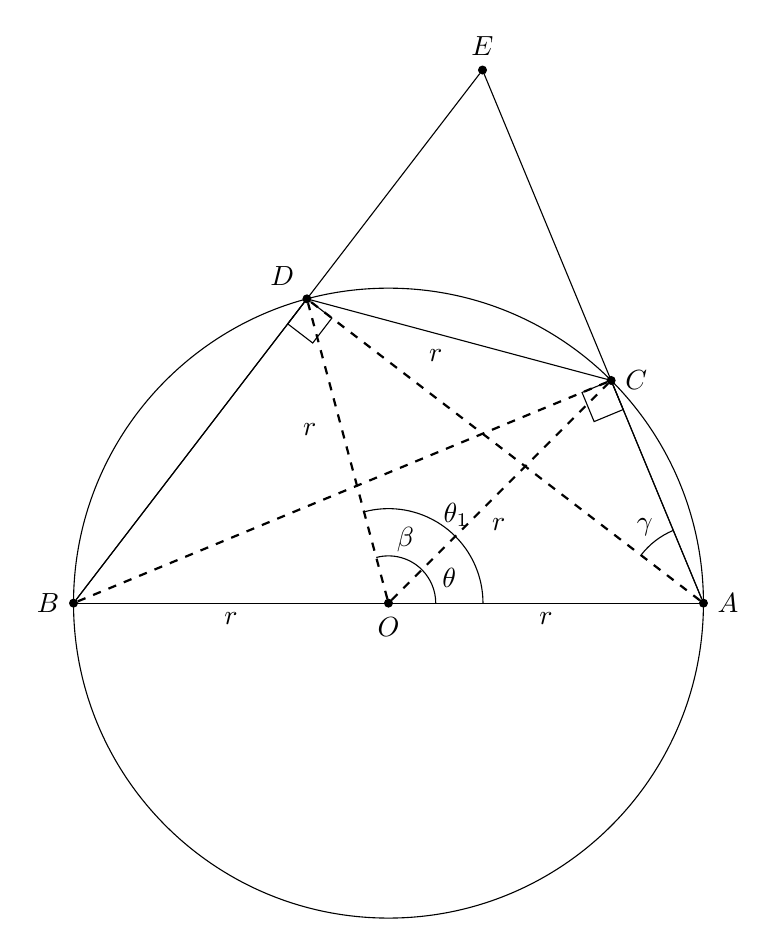
\begin{tikzpicture}
[scale =2,>=stealth,point/.style = {draw, circle, fill = black, inner sep = 1pt},]

\def\rad{2}
\coordinate [point, label={below: $O$ }] (O) at (0, 0);
\draw (O) circle (\rad);
\node (B) at (-2,0)[point,label=left :$B$] {};
\node (A) at (2,0)[point,label= right :$A$] {};
\node (C) at (1.414, 1.414)[point,label=right :$C$] {};
\node (D) at (-0.518, 1.932)[point,label= above left :$D$] {};
\node (E) at (0.597,3.385)[point,label= above :$E$] {};
\draw (A)--(B);
\draw (C)--(A);
\draw (B)--(D);
\draw (B)--(E);
\draw (C)--(D);
\draw (E)--(A);

\draw [thick,dashed](C)--(B);
\draw [thick,dashed](O)--(D);
\draw [thick,dashed](O)--(C);
\draw [thick,dashed](A)--(D);
\tkzMarkRightAngle[size=0.2](B,C,A)
\tkzMarkRightAngle[size=0.2](B,D,A)
\tkzMarkAngle[fill=orange!40,size=0.3cm,mark=](C,O,D)
\tkzLabelAngle[pos=0.4](C,O,D){$\beta$}
\tkzMarkAngle[fill=orange!40,size=0.5cm,mark=](C,A,D)
\tkzLabelAngle[pos=0.6](C,A,D){$\gamma$}
\tkzMarkAngle[fill=orange!40,size=0.3cm,mark=](A,O,C)
\tkzLabelAngle[pos=0.4](A,O,C){$\theta$}
\tkzMarkAngle[fill=orange!40,size=0.6cm,mark=](A,O,D)
\tkzLabelAngle[pos=0.7](A,O,D){$\theta_1$}

\node [above] at (-1,-0.2){$r$};
\node [above] at (1,-0.2){$r$};
\node [above] at (0.7,0.4){$r$};
\node [above] at (-0.5 , 1){$r$};
\node [above] at (0.3 ,1.47){$r$};
%\node [above right] at (0.4,-0.5){$\theta=\frac{2\pi}{n}$};
\end{tikzpicture}

\end{document}

